\documentclass{sig-alternate-05-2015}
\usepackage{graphicx}
\graphicspath{ {images/} }
\begin{document}

% Copyright
\setcopyright{acmcopyright}

\title{Modelling Relationships in Autonomous Systems and inter-domain Routing policies}

\numberofauthors{3} %  in this sample file, there are a *total*
% of EIGHT authors. SIX appear on the 'first-page' (for formatting
% reasons) and the remaining two appear in the \additionalauthors section.
%
\author{
% You can go ahead and credit any number of authors here,
% e.g. one 'row of three' or two rows (consisting of one row of three
% and a second row of one, two or three).
%
% The command \alignauthor (no curly braces needed) should
% precede each author name, affiliation/snail-mail address and
% e-mail address. Additionally, tag each line of
% affiliation/address with \affaddr, and tag the
% e-mail address with \email.
%
% 1st. author
\alignauthor Abhinav Agshikar\\
       \email{abhinav.agshikar\textsuperscript{1}}
% 2nd. author
\alignauthor
Sagar Thakkar\\
       \email{sagar.thakkar\textsuperscript{1}}
% 3rd. author
\alignauthor
Arnav Gupta\\
       \email{arnav.gupta\textsuperscript{1}}
}


\maketitle
\section{PROBLEM STATEMENT}
Internet Measurement - modeling relationships in Autonomous Systems (ASes) and Inter-domain routing policies using CAIDA dataset and RIPE Atlas. 

\begin{abstract}
In this two part project, we plan to understand the relationships between Autonomous Systems (ASes) on the Internet and derive inferences
between theoretical and practical routing scenarios. For the first part of the project, we use the March 2016 CAIDA Dataset  [3] that 
represents a theoretical model of the AS relationships using the now standard Gao-Rexford model  [1] and create
a graph visualization using Neo4j [4] graph database. We present our analysis using statistics obtained with this dataset and pick the top 100
mostly connected ASes and use them for further analysis. In the second part  of the project that we will progress next,
we will explore practical routing scenarios using RIPE Atlas framework by using probe nodes found in the first part and find out routing
instabilities at inter-AS routing level.

\end{abstract}

\keywords{Autonomous Systems; Gao-Rexford Model\footnote{@stonybrook.edu}; RIPE Atlas; BGP; Graph Database}

\section{Introduction}
\subsection{BGP and Autonomous Systems}
In the Internet, different ISPs communicate with each-other. These ISPs communicate with their customers using various Intra-domain routing protocols whose decision is made by the provider itself. They can decide the protocol based on their network traffic and distribution of customers in the geographical area (topology). However all these ISPs have to communicate with each other via a common protocol. This protocol which is agreed by the entire Internet community is called Border Gateway Protocol (BGP). The interdomain (exterior) routing paradigm is driven by the BGP communication between the Autonomous Systems (ASes). These Autonomous Systems are the exit point of a particular network driven by a network provider. These ASes communicate with other ASes based on certain policies. These policies are varied and is explained by now standard and accepted Gao - Rexford model.

\subsection{Gao - Rexford Model\textsuperscript{[1]}}
Generally while running a protocol to setup routes to the destination, it is typically done in a dynamic fashion via path vector-based implementation. However this protocol complexity lies in the set of routing policies each AS implements. To converge to a particular destination, there are often different ASes to traverse. A standard approach may be selecting the shortest path or the least cost path. However this is not true in all the cases, in practice the selection of ASes is based on various other factors including but not limited to financial policies between ISPs and amount of traffic to traverse the network. Due to this, there are always anomalies in the shortest path and the selected path in practical scenarios. Gao - Rexford model provides a set of guidelines that an AS can implement to set up its routing policies without coordination with other ASes and guarantee the convergence of path. This model gives us the ideal path between the ASes. We then compare the actual path and find anomalies in BGP routing in this project. We obtain the ideal connection details between ASes from CAIDA data set and the Actual connection using RIPE Atlas.

\subsection{CAIDA Dataset\textsuperscript{[4]}}
CAIDA stands for Center for Applied Internet Data Analysis. CAIDA curates datasets resulting from both active and passive Internet measurement and has been used
in several research papers. The dataset establishes relationships using the Gao-Rexford model. We use this information provided by CAIDA and obtain a list of ASes that are critical to the Internet infrastructure. Later we work to obtain the AS Topology map using this dataset.

\subsection{RIPE Atlas\textsuperscript{[5]}}
RIPE Atlas is a global, open, distributed Internet measurement platform, consisting of thousands of measurement devices that measure Internet connectivity in real time. Each AS has a probe sitting at the node to measure the network information. All these devices contribute to the Atlas community to share the information. We then use this information of ping and traceroute to identify the anomalies.
The RIPE Atlas has a number of restrictions with respect to the measurements that can be done-
\begin{enumerate}
\item No more than 100 simultaneous measurements for a single user
\item No more than 500 probes may be used per measurement
\item No more than 10 traceroute or ping UDMs can exist for a given target URL/IP for all users of the system. The condition does not apply to DNS measurements

\end{enumerate}
We plan to choose a set of Vantage points by picking up interesting ASes from list obtained from CAIDA.

\section{Problem Description}
From the early days of Internet, it has been constantly evolving. Now we see that millions of entities have been added over the period of time. The common man could only wonder how the existing entities connect with each other let alone the new ones. The protocol which has been assigned this responsibility is BGP. Although the routing of a packet as it happens it became increasingly clear to the entities that the current shortest-path routing is not sufficient to be able to manage the ever changing scenario which are constantly influenced by the operational, economic, and political factors involved in routing. The main driving force behind this modified decision making were the ISPs which began to change the routing configurations to manage the routing policies, which mean that the decision making done by the owners of the router which were managing the routes were changed and hence the routes which were exchanged between the neighbors were also different now. It was in the earlier days of BGP it followed a simple routing  path-vector protocol. It is just subsequently that so many changes have been made by the ISPs so that they are able to reduce the cost they bear for routing packets to and fro through their own network. The protocol which now exists for routing packets is completely changed and lot of modifications introduced that are not compatible with each other and one can observe several conflict in various ways. The main problem with these updations is that many of the changes can be highly unpredictable and many of them are involved in the decision process which is important for selection of routes. Some of the modifications are not even mentioned in the standard protocol specification. It has become increasingly difficult to keep track or make any predictions of any sort as to how the packet will route and which path it will take. Thus the complexity increasingly causes increase in problems which might include security problems or wrong configuration and also the several conflicts while interacting between router owned by different ISPs which could break the Internet infrastructure.


The most important responsibility of autonomous systems is to send and receive the information about network routing between different ASes. The information being exchanged also composes of information about the ASes which were being traversed in order to reach the intended destination (hop information). We require this information in order to develop the path which was actually taken by the packet in order to reach the destination. We can derive lot of other information about the reachability using which certain loops can be discarded and also the ISP specific policy decisions could be implemented and studied. It is very important to understand the basic fundamentals and how the model of network routing form the base for implementing security and improving the reliability and constantly evolve as currently the experiments done to understand the routing are done using simulations of the entire routing system. It is very difficult that any model can be proposed based on some simulation as it will not be based on real time data, as we already know that it is the ISPs are constantly trying to take benefit and reduce cost by tweaking routing policies for their router and many don’t even let the other companies know what actual routing policies they might have used for their routers. 

Discrepancies or anomalies are a day-to-day occurrence for the inter-network routing protocol. They could include anything from a misconfiguration in the infrastructure to an incorrect update being shared between the routers that could dangerously affect routing for particular regions. As a researcher thus it becomes a responsibility to understand and bring forth some of the routing anomalies that exist which can help us in understanding things like filtering, misdirection and interception. It entirely depends on the anomaly and which of the control/data plane. This detection can be done using a very sophisticated approach. It becomes very important to get the dataset from different ASes which form the key role in the routing of packets and which have more and more connections to other routers. It is the AS which has most number of probes is very important to study and understanding the routing the policies of such AS would help us find the anomalies that could help us the different policies employed by the ISPs. In order to find anomalies we need to be able to select the top ASes and to identify the anomalies at this ASes.

In this project, we have thought of analyzing AS routing scenarios by looking at theoretical standard model i.e. Gao Rexford model versus practical routing scenarios obtained by traceroutes via ATLAS RIPE APIs. The motivation for this is to ensure authenticity and consistency on the Internet. Initially we present our analysis on the well known and heavily used CAIDA AS dataset and then proceed to its visualization using graph database. We try to derive inferences on the nature of the AS graph existing on the Internet using this dataset and identify possible ASes and probes that we can use for the next part of the project.
\section{Solution Methodology}

We decided to split our project into two parts: AS Structure Visualization and AS BGP practical routing. For part 1, we used the CAIDA dataset to obtain AS relationships existing as of March 2016. We obtained two files - AS Rel file that contains AS-AS relationship mapping which can either be Peer to Peer or Provider to Customer. The other file contained a list of existing connections between ASes from where we identified most prominent ASes that has maximum connections. We retrieved a list of 100 most connected list of ASes and found their corresponding relationships in the first file. This gave us a list of 28846 unique ASes that we visualized along with their existing Peer-Peer and Provider-Customer relationships using Neo4j.

For remaining portion of the project, we will work on RIPE Atlas traceroutes by using ASes and their corresponding Vantage points identified in part 1. We discussed these details in our Future Work section.

\section{Evaluation and Results}
\subsection{Analysis on CAIDA Dataset}
We first performed analysis on entire CAIDA dataset as of March 2016. The summary of this set is listed below:

\begin{center}
\begin{tabular}{ |c|c|c| } 
 \hline
 No of Unique ASes & 53537 \\ 
 \hline
 No of Links & 406401 \\ 
 \hline
\end{tabular}
\\Table 1: Statistics of Complete Dataset\\
\end{center}

We next narrowed this dataset by using the top 100 most connected ASes. We list summary and top 5 most connected Ases these below:

\begin{center}
\begin{tabular}{ |c|c|c| } 
 \hline
 No of Unique ASes & 28846 \\ 
 \hline
 No of Links & 68712 \\ 
 \hline
\end{tabular}
\\Table 2: Statistics of Reduced Dataset\\
\end{center}



\begin{center}
\begin{tabular}{ |c|c|c| } 
 \hline
ASN &  Name & Country \\
 \hline
ASN3356 &  Level 3 Communications, Inc. & USA \\
 \hline
ASN174 & Cogent Communications & USA \\
\hline
ASN1299 & TeliaSonera AB & Europe \\
\hline
ASN2914 & NTT America, Inc. & USA \\
\hline
ASN3257 & Tinet Spa & HongKong \\
\hline
\end{tabular}
\\Table 3: Top 5 most connected ASes\\
\end{center}
\begin{center}
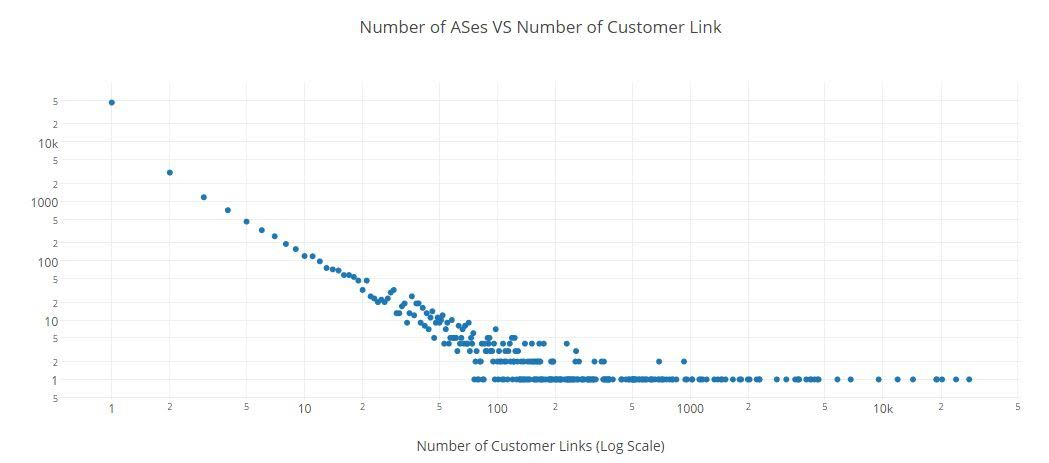
\includegraphics[scale=0.2]{graph1}\\
Fig 1. Scatter Plot of AS vs Number of links\\
\end{center}
The scatter plot above indicates that there are very few nodes having huge number of links (Peer-Peer and Provider-Customer). Around 15000 ASes have only one link while the highest number of links were around 28000.
\subsection{AS Relationship Visualization and Inferences}
Now we used Neo4j which is a graph database for visualizing these ASes. We created two CSVs containing the two relationships i.e.
Provider to Customer and Peer to Peer. We initially created the total list of 28846 nodes in the database and then input the relationships files.
\begin{center}
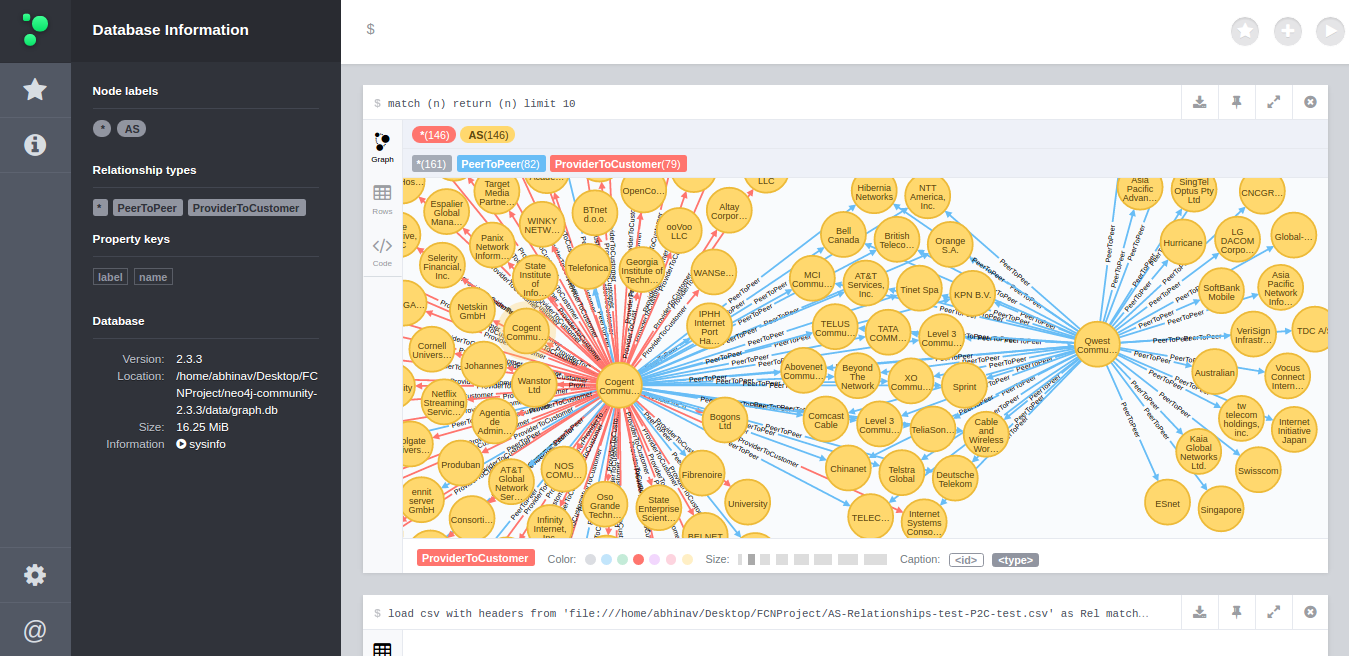
\includegraphics[scale=0.18]{graph2}\\
Fig 2. Visualization of Cogent and Qwest Communication ASes\\
\end{center}

\begin{center}
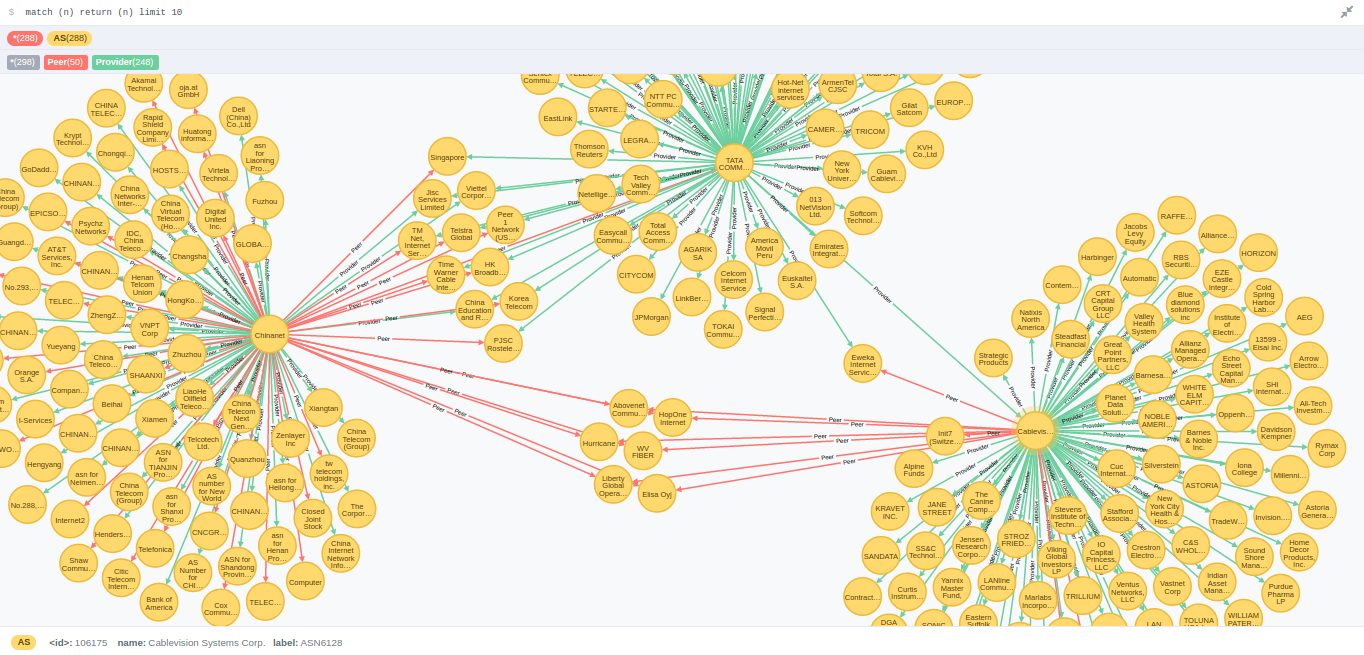
\includegraphics[scale=0.18]{graph3}\\
Fig 3. Visualization of ChinaNet vs Cablevision vs Tata Comm (US) \\
\end{center}
One of the interesting results that we could see is that the more highly linked ASes have 
very few Peer-Peer relationships with other ASes compared to a larger portion of Provider-Customer relationships.

\subsection{RIPE Atlas}
Amongst the top 100 highly connected list of ASes, we identified three particularly interesting ones that can be helpful in our further
analysis with RIPE Atlas -
AS6128: Cablevision Systems, AS6453: Tata Comm (US), AS4134: ChinaNet. For these three ASes, we found existing Internet Measurement
probes as listed in the summary table below. We will use these measurement ids as our Vantage Points for our next experiments.
\begin{center}
\begin{tabular}{ |c|c|c| } 
\hline
ASN &  Name & Atlas Probe IDs \\
 \hline
AS6453 &  Tata Comm (US) INC & 19797 \\
 \hline
AS6128 &  Cablevision Systems Corp. & 23478,22723, .. \\
 \hline
AS4134 &  ChinaNet & 23846,15504, .. \\
 \hline
 \end{tabular}
 \\Table 4: Vantage Points\\
\end{center}

\section{Future Work}
For the next part of our project, we will continue working on ATLAS RIPE. We have the connectivity information of the ASes which we will compare with the traceroute and ping responses dump available on the RIPE Atlas website for the Probe IDs corresponding to those ASes.
\begin{enumerate}
\item Use RIPE ATLAS ping and traceroute dump for the identifying the anomalies in the inter AS routing. This we plan to do by comparing the connectivity details we obtained for different vantage points in part 1 of the project. 
\item The anomalies which we plan to work upon includes but not limited to Identifying the bogus prefixes in the traceroute and mismatch between the Gao - Rexford model solution provided by the CAIDA dataset and the measurement information we obtained from the ATLAS dataset.


\end{enumerate}

\section{Acknowledgements}
We would like to thank Professor Aruna for her involvement in constant discussions through the progress of this project. We would also like to thank Professor Phillipa for her feedback on Internet Measurement and possible applications areas for RIPE Atlas.



\section{References}
\noindent1. ``Stable Internet Routing without Global co-ordination" - Lixin Gao, Jennifer Rexford\\
2. ``Investigating Interdomain Routing Policies in the Wild'' - Ruwaifa Anwar, Haseeb Niaz, et al\\
3. CAIDA datasets - http://data.caida.org/datasets \\
4. Neo4j Graph Database - http://neo4j.com\\
5. RIPE Atlas https://atlas.ripe.net\\
\end{document}
